\documentclass[a4paper]{article}
\usepackage{polski}
\usepackage{geometry}[top=2cm, left = 2.5 cm, right = 2.5cm]
\usepackage{graphicx}
\usepackage{float}
\graphicspath{{./images/} }
\title{
	\textbf{Zastosowanie systemów wbudowanych}\\
	\textit{Raspberry Pi - Telegram Bot i web-aplikacja dla śledzenia klimatu otoczenia}
	}
\date{}

\begin{document}
\begin{table}
	\vspace{-2cm}
	\begin{tabular}{rl}
		Autorzy & \\
			\hline
		Kostiukov Oleksii 	& 231972\\
		Uladzimir Lipski	& 238961\\
		Vikatr Hasiul 		& 231862\\[0.4cm]
			\hline
		Prowadzący 	& Dr inż. Marek Woda \\
		Termin		& Środa, godzina: 13:15\\
	\end{tabular}
\end{table}

{\let\newpage\relax\maketitle}
\maketitle
\thispagestyle{empty} %no page number for this page

\maketitle
\newpage
\section{Cel projektu}
	Celem danego projektu jest wykorzystanie platformy \textit{Raspberry} 
	do realizacji \textit{Telegram bot'u} oraz punktu pomiarowego.

	\paragraph{Telegam bot} jest aplikacją wykorzystującą interfejs aplikacji \textit{Telegram}
	w celu komunikacji z wybranymi użytkownikami (którzy posiadają możliwość komunikacji ze stworzonym
	\textit{bot'em}).

	\paragraph{Punkt pomiarowy.} Platforma \textit{Raspberry} umożliwia podłączenie licznych
	czujników, dane z których można gromadzić na urządzeniu lub wysyłać do serwerów zdalnych.
	W danym projekcie zostaną podłączone czujniki:
	\begin{enumerate}
		\item temperatury,
		\item wilgotności,
		\item światła
	\end{enumerate}
	dane z których będą przechowywane na urządzeniu w celu przetwarzania i 
	wyświetlania na stronie \textbf{WEB} w postaci interaktywnego wykresu.
	
	Dodatkowo dany zbiór danych zostanie wykorzystany przez \textit{Telegram bot}
	w celu powiadomienia użytkownika o aktualnych danych.

\section{Implementacja}
    \subsection{Pobór danych za pomocą czujników}
    \subsection{Podłączenie do sieci Internet}
    \subsection{Komunikacja z Telegram botem}
    \subsection{Aplikacja internetowa}

    \subsubsection{Cel aplikacji internetowej}
        Celem aplikacji internetowej jest wizualizacja danych, pobranych za pomocą czujników platformy Raspberry Pi. Dane są wyświetlane za pomocą wykresów, a mianowicie histogramów. Wykresy pokazują jak często występuje każdy z zadanych zakresów temperatury, natężenia światła albo wilgotności. Wykresy w przeglądarce muszą być odświeżone asynchronicznie od razu po zmianie pliku, które te dane przechowuje.
        
        \begin{figure}[H]
            \centering
            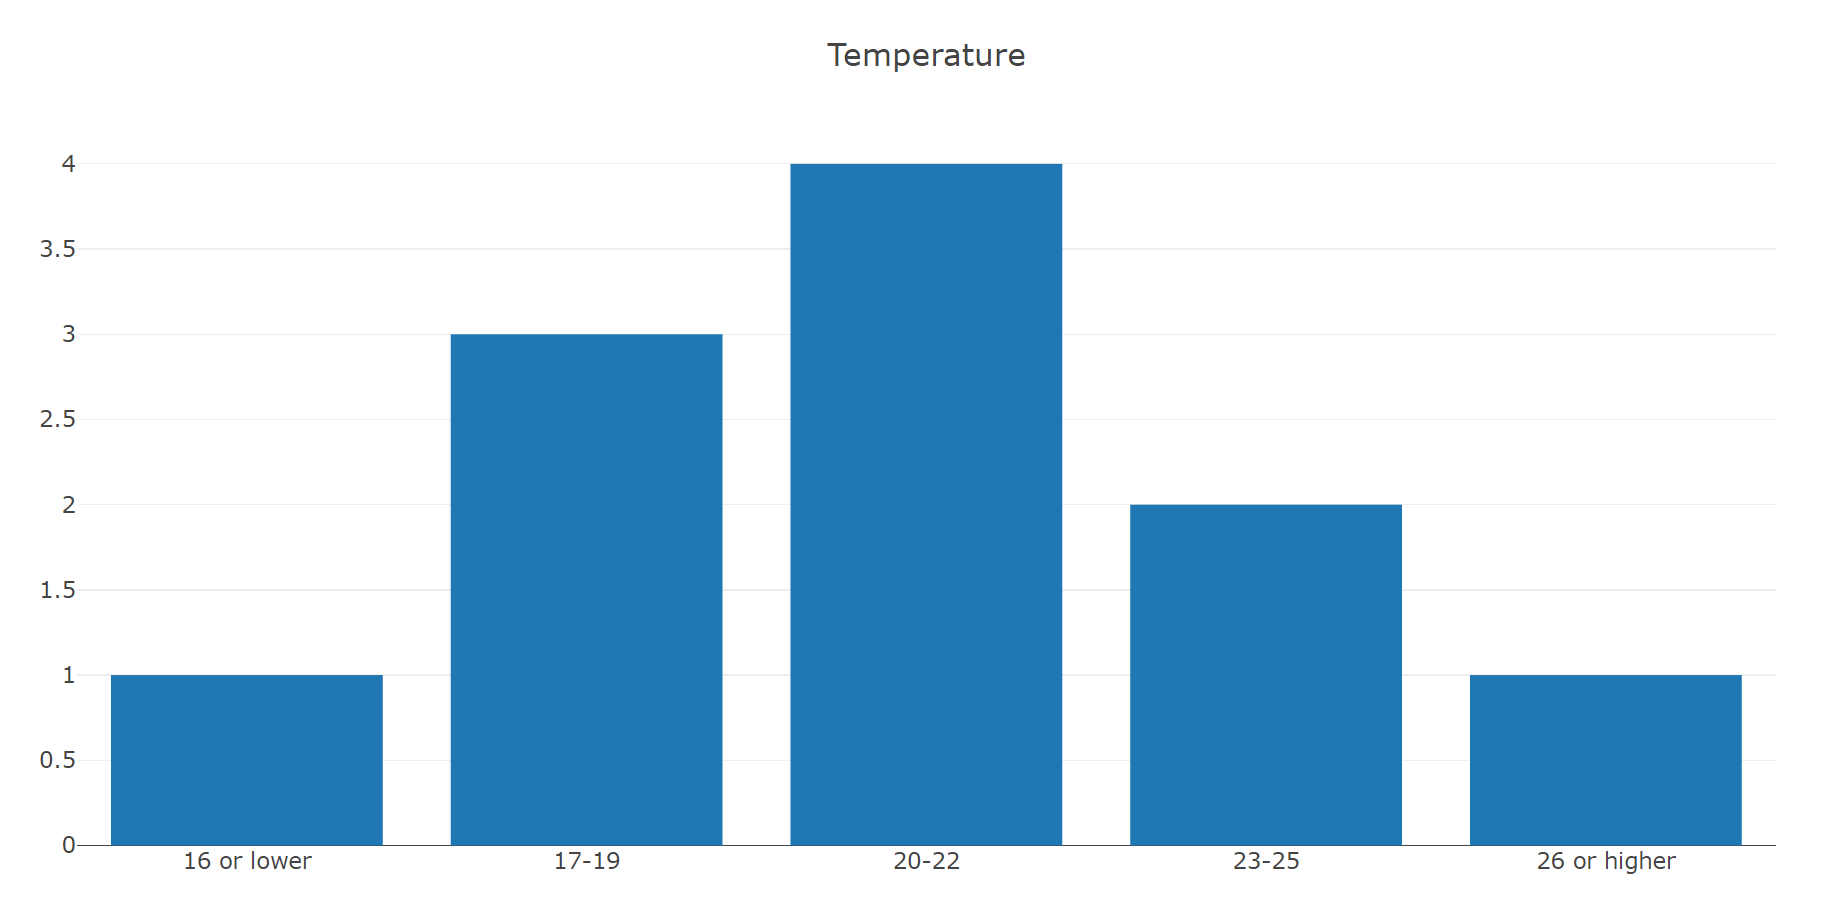
\includegraphics[scale=0.4]{exampleChart}
            \caption{Histogram temperatury}
        \end{figure}
        
        \subsubsection{Wybór platformy web-serwera}
        Aplikacja internetowa jest stworzona za pomocą frameworku Flask. Flask - framework do tworzenia aplikacji internetowych w języku Python, należący do kategorii tak zwanych mikroframeworkow - minimalistycznych ram aplikacji internetowych, które celowo zapewniają tylko najbardziej podstawowe funkcje.
        
        Zaletami frameworku sa:
        \begin{enumerate}
            \item Elastyczność
            \item Minimalistyczność bez straty mocy
            \item Prosty w nauce i obsłudze
            \item Łatwe rutowanie adresów URL
            \item Łatwa rozszerzalność
        \end{enumerate}
    
    \subsubsection{Generowanie wykresów w przeglądarce}
    
        Dla utworzenia wykresów w przeglądarce używana jest biblioteka Plotly, napisana w języku JavaScript. Biblioteka pozwala na utworzenie wykresu wybranego typu, który dla danej aplikacji jest typem 'bar', odpowiadającym histogramowi. Dane dla wykresów są przekazywane od serwera do przeglądarki jako odpowiedz na żądanie HTTP.
        
        Funkcja do utworzenia wykresu przyjmuje jako parametr "id" elementu z tagiem "div", w którym będzie się znajdować dany wykres.
        
        \begin{figure}[H]
            \centering
            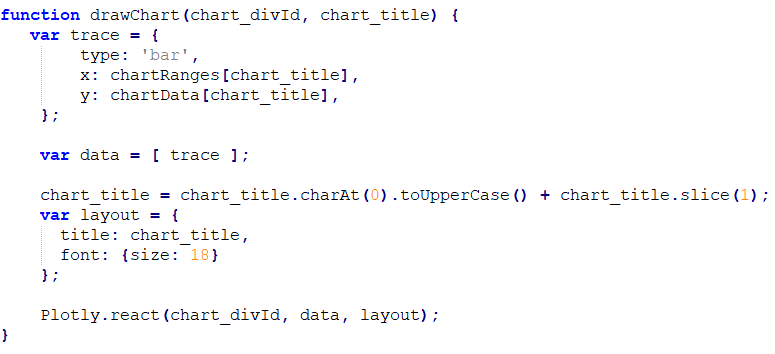
\includegraphics{images/plotlyExample.png}
            \caption{Funkcja do tworzenia histogramu za pomocą biblioteki Plotly.js}
        \end{figure}
        
        Dane z serwera są przekazywane w postaci tablicy. Dodatkowym zadaniem skryptu w języku JavaScript jest kategoryzowanie (rozrzucenie) danych dla różnych zakresow, zanim wykres będzie stworzony.
        
        Wartości dla osi X są nazwami zakresów, do których może należeć wartość przekazana z serwera. Dane zakresy są zdefiniowane są statyczne i zadeklarowane na samym początku skryptu.
        
        \begin{figure}[H]
            \centering
            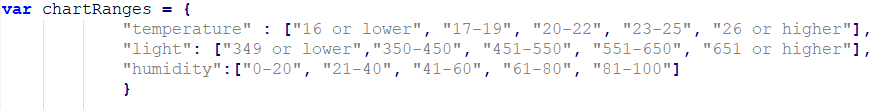
\includegraphics[scale=0.9]{images/chartRanges.png}
            \caption{Zdefiniowany zakresy w skrypcie JavaScript}
        \end{figure}
    
    \subsubsection{Asynchroniczne wczytywanie danych z pliku}
    
        Dane, pobrane z czujników za pomocą platformy Raspberry Pi, są przechowywane w pliku z rozszerzeniem ".csv". Dla asynchronicznego wczytywania danych z pliku używana jest biblioteka "watchdog", napisana w języku Python.
        
        Celem biblioteki jest monitorowanie wybranych plików. Wybór plików odbywa się za pomocą wyrażeń regularnych. Jeżeli jakiś z monitorowanych plików zostaje zmieniony, to do serwera jest wysyłany sygnał. Do obsługi różnego rodzaju sygnałów używana jest biblioteka "flask\_socketio".
        
        Dla każdego sygnału mogą być zdefiniowane osobne funkcje. Na przykład jeżeli monitorowany plik został zmieniony i zapisany, to do serwera zostaje wysłany sygnał, który wywołuje funkcje "on\_modified", która była zdefiniowana dla śledzenia danego sygnału.
        
        Po otrzymaniu sygnalu funkcja "on\_modified" linijka po linijce wczytuje dane z pliku dlatego, żeby te dane wysłać do przeglądarki.
        
        Monitorowanie pliku jest osobna funkcja i to monitorowanie musi się odbywać w osobnym wątku, żeby nie blokować aplikacji.
        
        \begin{figure}[H]
            \centering
            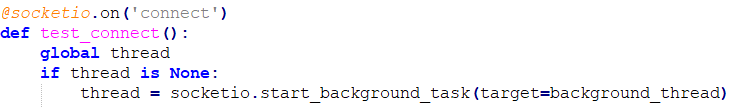
\includegraphics{images/csvWatcher.png}
            \caption{Początek wątku, monitorującego zmianę w pliku}
        \end{figure}
    
    \begin{figure}[H]
        \centering
        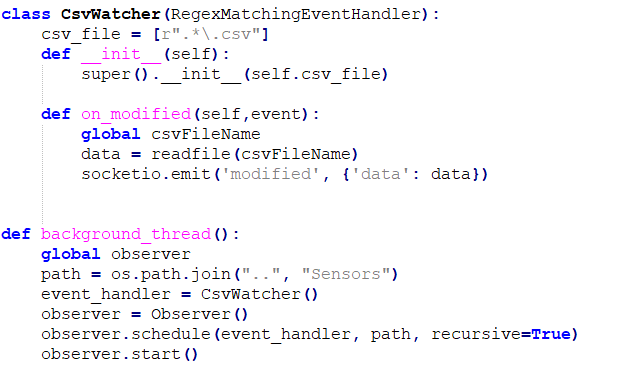
\includegraphics{images/csvWatcher2.png}
        \caption{Funkcja reagująca na sygnał po zmianie pliku}
        \label{fig:mesh1}
    \end{figure}
    
    \subsubsection{Asynchroniczne odświeżanie wykresów w przeglądarce}
        
        Język JavaScript również pozwala na zdefiniowanie socket'ów. Celem socketów jest asynchroniczna obsługa sygnałów, wysłanych z serwera.
        
        Jak jest pokazane na rysunku \ref{fig:mesh1}, po zmianie pliku serwer wywołuje funkcje "on\_modified", która wczytuje plik i wysyła sygnał z wczytanymi danymi do przeglądarki.
        Po otrzymaniu sygnału skrypt JavaScript odświeża wykresy w przeglądarce.
        
        \begin{figure}[H]
            \centering
            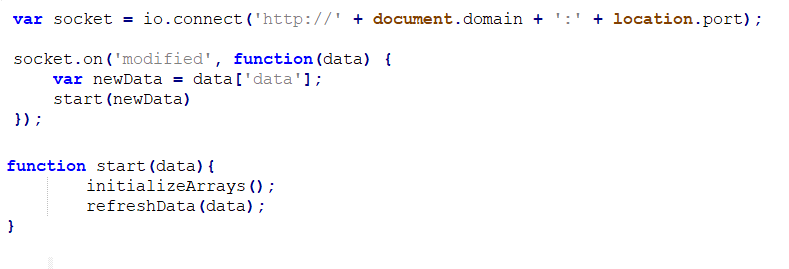
\includegraphics{images/socketInJs.png}
            \caption{Funkcja odświeżająca wykresy po otrzymaniu sygnału z serwera}
        \end{figure}
        
    \subsubsection{Dostęp do aplikacji w sieci prywatnej}

        Dla uruchamiania aplikacji ktora będzie dostępna w sieci prywatnej, potrzebne jest odpowiednie ustawienie parametru "host". Jeżeli parametr "host" będzie ustawiony na "0.0.0.0", to aplikacja będzie dostępna pod adresem, którym jest zewnętrzny adres IP. Adres IP można sprawdzić na przykład na stronie https://www.myip.com/.
        
        \begin{figure}[H]
            \centering
            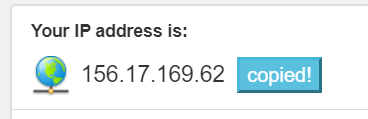
\includegraphics{images/myipaddress.png}
            \caption{Adres IP na stronie https://www.myip.com/}
        \end{figure}
        
        \begin{figure}[H]
            \centering
            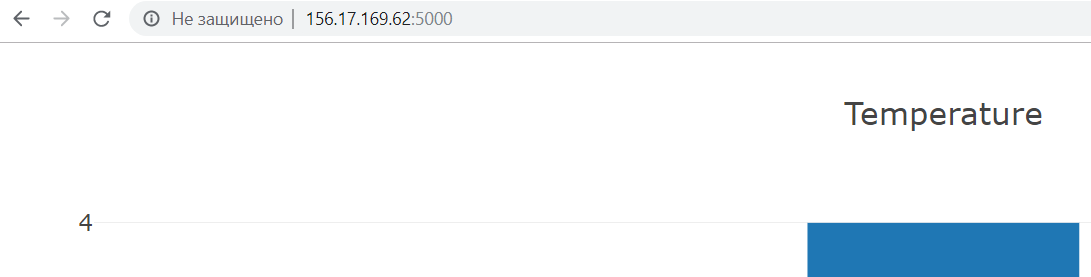
\includegraphics[scale=0.7]{images/runningApp.png}
            \caption{Uruchomiona aplikacja pod zewnętrznym adresem IP}
        \end{figure}
        
\end{document}